\documentclass[cmbright]{staauth}

\usepackage{amssymb, amsmath, latexsym, array, morefloats, epsfig, rotating, graphicx}
\usepackage{subfigure, url, mathtools, enumerate, wasysym, threeparttable, lscape}
\usepackage{natbib,color}
\usepackage{bm, bbm,epstopdf}
\usepackage{xr, zref, hyperref}
\usepackage{cprotect}

%\usepackage[nomarkers]{endfloat}

\newcommand{\var}{\mathrm{var}}
\newcommand{\cov}{\mathrm{cov}}
\newcommand{\E}{\mathrm{E}}
\newcommand{\tr}{\mathrm{tr}}

% if variable blind is undefined, assume it is 0
\makeatletter
\@ifundefined{blind}{\def\blind{0}}{}
\makeatother

% if not blinded, reference unblinded appendix
\if0\blind
{
  \externaldocument{psokrigingapp}
}\fi

% if blinded, reference blinded appendix
\if1\blind
{
  \externaldocument{psokrigingappblind}
}\fi


\begin{document}
\if0\blind
{
  \runninghead{M Simpson}{AT-PSO for Spatial Design}
  \title{Adaptively-Tuned Particle Swarm Optimization with Application to Spatial Design}
  \author{Matthew Simpson\affil{a}\corrauth, Christopher K. Wikle\affil{a}, Scott H. Holan\affil{a,b}}
  \address{\affilnum{a}Department of Statistics, University of Missouri, 146 Middlebush Hall, Columbia, MO 65211-6100\\
\affilnum{b}U.S. Census Bureau, 4600 Silver Hill Road, Washington, D.C. 20233-9100}
  \corremail{themattsimpson@gmail.com}
  \received{00 Month Year}
  \accepted{00 Month Year}
}\fi

\if1\blind
{
  \runninghead{}{AT-PSO for Spatial Design}
  \title{Adaptively-Tuned Particle Swarm Optimization with Application to Spatial Design}
  \author{}
  \address{}
  \corremail{}
  \received{}
  \accepted{}
}\fi
\begin{abstract}
Particle swarm optimization (PSO) algorithms are a class of heuristic optimization algorithms that are attractive for complex optimization problems. We propose using PSO to solve spatial design problems, e.g. choosing new locations to add to an existing monitoring network. Additionally, we introduce two new classes of PSO algorithms that perform well in a wide variety of circumstances, called adaptively-tuned PSO and adaptively-tuned bare bones PSO. To illustrate these algorithms, we apply them to a common spatial design problem: choosing new locations to add to an existing monitoring network. Specifically, we consider a network in the Houston, TX area for monitoring ambient ozone levels, which have been linked to out-of-hospital cardiac arrest rates.
\end{abstract}
\keywords{geostatistics; kriging; optimal design; optimization; particle swarm; spatial prediction}
\maketitle

\section{Introduction}
A common step in many statistical problems is the optimization of some objective function. Gradient-based algorithms solve many of these problems efficiently, but some problems are too difficult to solve efficiently with these methods. For example, in spatial design problems, the objective function consists of some design criterion typically related to the variability of predictions, which is a complex function of the design points often with multiple local and global optima, and this function may be defined over a complex domain. Gradient-based methods are typically inefficient for these problems and often fail. We propose using particle swarm optimization (PSO) as a more robust alternative for design problems and more generally for other statistical optimization problems where gradient-based methods fail. We illustrate the usefulness of PSO as a tool for solving design problems by applying several PSO algorithms to choosing a set of new monitoring locations for ozone in Harris County, Texas (USA), where Houston is located. Ambient ozone levels have been linked to cardiac arrest, \cite{ensor2013case}, and ozone monitoring is an essential tool for determining when and where populations are at risk. For a fixed network size or cost, optimized network design improves the quality of information available to policy makers using the network.

Particle swarm optimization (PSO) refers to a large class of heuristic optimization algorithms that that rely on an analogy with animal flocking behavior and are typically more robust than many alternatives; \cite{clerc2002particle,blum2008swarm,clerc2010particle}. This robustness makes them attractive for more difficult optimization problems such as the design problems we discuss, especially when near optimal solutions are tolerable. We introduce two new classes of PSO algorithms, called adaptively-tuned PSO (AT-PSO), and adaptively-tuned bare bones PSO (AT-BBPSO), which exploit an analogy with a class of adaptive Markov chain Monte Carlo algorithms in order to tune a crucial parameter of the algorithm adaptively based on the state of the particle swarm. We show that the resulting algorithms are competitive with, and in some cases significantly better than, many PSO alternatives.

The remainder of the paper is organized as follows. Section \ref{sec:pso} introduces various PSO, AT-PSO, and AT-BBPSO algorithms, whereas Section \ref{sec:psocompare} briefly discusses the results of a simulation study comparing them. Section \ref{sec:spatialdesign} introduces a generic spatial design problem and the Houston area ozone problem as an instance of that problem, and compares several PSO algorithms and some alternatives to solving the problem. Finally, Section \ref{sec:discuss} discusses our results and concludes. 

\section{Particle swarm optimization}\label{sec:pso}
We briefly describe PSO here; see \cite{blum2008swarm} for a comprehensive introduction, \cite{clerc2010particle} for additional details, and \cite{clerc2011spso} for good default versions of the algorithm. Suppose that we wish to minimize some objective function $Q(\bm{\theta}):\Re^D\to\Re$. Let $i=1,2,\dots,n$ index a set of particles over time, $k=1,2,\dots,K$, where in every period each particle consists of a location $\bm{\theta}_i(k)\in \Re^D$, a velocity $\bm{v}_i(k) \in \Re^D$, a personal best location $\bm{p}_i(k)\in\Re^D$, and a group best location $\bm{g}_i(k)\in\Re^D$. Here we mean ``best'' in the sense of minimizing $Q$, so $Q(\bm{p}_i(k)) \leq Q(\bm{\theta}_i(l))$ for any $k\geq l$. The group best location is defined with respect to some neighborhood $\mathcal{N}_i$ of particles for particle $i$; that is, $\bm{g}_i(k) = \arg\min_{\{\bm{p}_j(k)|j\in\mathcal{N}_i\}}Q(\bm{p}_j(k))$. In the simplest case where the entire swarm is the neighborhood of each particle, $\bm{g}_i(k)\equiv \bm{g}(k) = \arg\min_{\{\bm{p}_j(k)|j\in 1:n\}}Q(\bm{p}_j(k))$. The generic PSO algorithm updates each particle $i$ as follows:
\begin{align}\label{eq:pso}
\bm{v}_i(k+1) &= \omega \bm{v}_i(k) + \phi_1 \bm{r}_{1i}(k)\circ\{\bm{p}_i(k) - \bm{\theta}_i(k)\} + \phi_2 \bm{r}_{2i}(t)\circ\{\bm{g}_i(k) - \bm{\theta}_i(k)\},\nonumber\\
\bm{\theta}_i(k+1) &= \bm{\theta}_i(k) + \bm{v}_i(k+1),\nonumber\\
\bm{p}_i(k+1) &= \begin{cases} \bm{p}_i(k)   & \mbox{if }\  Q(\bm{p}_i(k)) \le Q(\bm{\theta}_i(t + 1))\\
                               \bm{\theta}_i(k+1) & \mbox{otherwise},
\end{cases}\nonumber\\
\bm{g}_i(k+1) &= \arg\min_{\{\bm{p}_j(k+1)|j\in\mathcal{N}_i\}}Q(\bm{p}_j(k+1)),
\end{align}
where $\circ$ denotes the Hadamard (element-wise) product, $\bm{r}_{1i}(k)$ and $\bm{r}_{2i}(k)$ are each vectors of $D$ random variates independently generated from the $U(0,1)$ distribution, and $\omega>0$, $\phi_1>0$, and $\phi_2>0$ are user-defined parameters. The term $\omega \bm{v}_i(k)$ controls the particle's tendency to keep moving in the direction it is already going, so $\omega$ is called the inertia parameter. Similarly $\phi_1 \bm{r}_{1i}(k)\circ\{\bm{p}_i(k) - \bm{\theta}_i(k)\}$ controls the particle's tendency to move towards its personal best location while $\phi_2 \bm{r}_{2i}(k)\circ\{\bm{g}_i(k) - \bm{\theta}_i(k)\}$ controls its tendency to move toward its group best location, so $\phi_1$ and $\phi_2$ are called the cognitive correction factor and social correction factor, respectively; \cite{blum2008swarm}. This version of PSO is equivalent to \cite{clerc2002particle}'s constriction type I particle swarm, though there are many other variants. One default choice sets $\omega = 0.7298$ and $\phi_1 = \phi_2 = 1.496$, \cite{clerc2002particle}, while another sets $\omega = 1/(2\ln 2)\approx 0.721$ and $\phi_1=\phi_2=1/2 + \ln 2\approx 1.193$, \cite{clerc2006stagnation}.

Any PSO variant can also be combined with various neighborhood topologies that control how the particles communicate with each other. The default global topology allows each particle to see each other particle's previous best location for the social components of their respective velocity updates, but this can cause inadequate exploration and premature convergence. Alternative neighborhood topologies force each particle to communicate with fewer of the other particles. In addition to the global topology, we use a variant of the stochastic star topology from \cite{miranda2008stochastic}. Each particle informs itself and $k$ random particles from the swarm, sampled with replacement during initialization of the algorithm. On average this implies that each particle is informed by $k$ particles, though a small number of particles will often be informed by many of the other particles.

Bare bones PSO (BBPSO) is a variant of PSO introduced by \cite{kennedy2003bare} that strips away the velocity term. Let $\theta_{ij}(k)$ denote the $j$th coordinate of the position for the $i$th particle in period $t$, and similarly for $p_{ij}(k)$ and $g_{ij}(k)$. Then the BBPSO algorithm obtains a new position coordinate $\theta_{ij}$ via
\begin{align}\label{eq:bbpso}
\theta_{ij}(k+1) \sim N\left(\frac{p_{ij}(k) + g_{ij}(k)}{2}, |p_{ij}(k) - g_{ij}(k)|^2\right).
\end{align}
The updates of $\bm{p}_i(k)$ and $\bm{g}_i(k)$ are the same as in \eqref{eq:pso}. Several modifications can be made to PSO and BBPSO to improve performance, and Section \ref{app:psodetail} of the supporting materials details which ones we use. In the next two subsections we introduce two novel algorithms: adaptively-tuned BBPSO and adaptively-tuned PSO respectively.

\subsection{Adaptively-tuned BBPSO}\label{subsec:ATBBPSO}
BBPSO adapts the effective size of the swarm's search space over time through the variance term, $|p_{ij}(k) - g_{ij}(k)|^2$. As the personal best locations of the swarm move closer together, these variances decrease and the swarm explores locations that are closer to known high value areas in the space. This behavior is desirable, but the adaptation is forced to occur only through personal and group best locations. In order to allow the algorithm to adapt in a more flexible manner, we modify the BBPSO variance to $\sigma^2(k)|p_{ij}(k) - g_{ij}(k)|^2$ and tune $\sigma^2(k)$ in a manner similar to how the proposal standard deviation is tuned in adaptive random walk Metropolis MCMC algorithms; \cite{andrieu2008tutorial}. Define the improvement rate of the swarm in period $t$ as $R(k) = \#\left\{i:Q(\bm{p}_i(k)) < Q(\bm{p}_i(k-1))\right\}/n$ where $\#A$ denotes the cardinality of the set $A$. Adaptively-tuned BBPSO (AT-BBPSO) compares $R(k)$ to a target improvement rate $R^*$ and adjusts $\sigma^2(k)$ accordingly. Specifically AT-BBPSO updates the swarm's personal best and group best locations as in \eqref{eq:pso}, then updates particle locations as follows:
\begin{align}\label{eq:at-bbpso}
\theta_{ij}(k+1) &\sim t_{df}\left(\frac{p_{ij}(k) + g_{ij}(k)}{2}, \sigma^2(k)|p_{ij}(k) - g_{ij}(k)|^2\right),\nonumber\\
\log \sigma^2(k+1) &= \log\sigma^2(k) + c\{R(k+1) - R^*\},
\end{align}
where $df$ is a user chosen degrees of freedom parameter and $c$ is a user specified parameter that controls the speed of adaptation. We use a $t$ kernel parameterized in terms of location and scale parameters with $df=1$ instead of a Gaussian because this works well with adaptively tuning $\sigma^2(k)$. Setting the target rate from $R^*=0.3$ to $R^*=0.5$ tends to yield AT-BBPSO algorithms that work well, which is unsurprising given that random walk Metropolis MCMC algorithms work best with $R^*$ in a similar range; \cite{gelman1996efficient}. The parameter $c$ controls the speed of adaptation so that larger values of $c$ cause the algorithm to adapt $\sigma^2(k)$ faster. We find that $c=0.1$ works well with our other parameter settings, though anything within an order of magnitude yields similar results and in our experience with these algorithms, there does not appear to be much to gain from optimizing the choice of this parameter. We use $\sigma^2(0)=1$ to initialize the algorithm at the standard BBPSO algorithm. 

Both using a $t$ kernel and adding a fixed scale parameter have been discussed in the BBPSO literature, but as \cite{kennedy2003bare} notes, in the standard BBPSO setting $\sigma^2=1$ yields the best algorithms. \cite{hsieh2010modified} propose a variant that deterministically changes $\sigma^2$, starting it below one and gradually increasing it until a final set of iterations with $\sigma^2=1$. They also suggest tuning $\sigma^2$ dynamically, but give no suggestion for how to do this.

AT-BBPSO is able to adapt its value ``on the fly'' based on local knowledge about the objective function. If too much of the swarm is failing to find new personal best locations, AT-BBPSO proposes new locations closer to known high value areas. If too much of the swarm is improving, AT-BBPSO proposes locations farther away from these areas in an effort to make larger improvements. This ability to adapt to local information about the objective function allows AT-BBPSO to more quickly traverse the search space towards the global optimum, though by using local information AT-BBPSO does risk premature convergence to a local optimum. The adaptively-tuned component of AT-BBPSO can also be combined with most BBPSO variants, some of which are outlined in Section \ref{app:psodetail} of the supporting materials. In Section \ref{sec:psocompare} we conduct a simulation study on several test functions that compares AT-BBPSO variants to other PSO and BBPSO variants in order to justify the parameter settings discussed above and demonstrate AT-BBPSO variants are attractive PSO algorithms. In particular, AT-BBPSO typically drastically improves on BBPSO, and for the most difficult objective functions, the best algorithms are AT-BBPSO variants.

\subsection{Adaptively-tuned PSO}\label{sec:AT-PSO}
In AT-BBPSO variants, the parameter $\sigma(k)$ partially controls the effective size of the swarm's search area, and we tune this parameter based on how much of the swarm is finding new personal best locations. In standard PSO the inertia parameter, denoted by $\omega$ in \eqref{eq:pso}, is roughly analogous to $\sigma^2$ in BBPSO. It controls the effective size of the swarm's search area by controlling how the magnitudes of the velocities evolve over time. We can use the mechanism we used to tune $\sigma^2(k)$ in AT-PSO to tune $\omega(k)$. Formally, AT-PSO is the same as PSO in \eqref{eq:pso}, but at the end of an iteration it adds a step to update $\omega(k)$ via
\begin{align}\label{eq:atpso}
\log\omega(k+1)& = \log\omega(k) + c \{R(k+1) - R^*\},
\end{align}
where $R(k)$ is the improvement rate of the swarm in iteration $t$, $R^*$ is the target improvement rate, and $c$ controls how much $R(k)$ changes on a per iteration basis. Again, we find that target rates from $R^*=0.3$ to $0.5$ work well for AT-PSO. The value of $c$ controls the speed of adaptation. We use $c=0.1$ as a default value and in simulations (not reported here), we find that the gains from optimizing $c$ appear to be small. This step can be combined with almost any PSO variant, and we combine it with each of the modifications listed in Section \ref{app:psodetail} of the supporting materials.

The idea of time-varying $\omega(k)$ has been in the PSO literature for some time. An early suggestion was to set $\omega(0)=0.9$ and deterministically decrease it until it reaches $\omega(k)=0.4$ after the maximum number of iterations allowed; \cite{eberhart2000comparing}. In particular, \cite{tuppadung2011comparing} suggest defining $\omega(k)$ via the parameterized inertia weight function $\omega(k) = 1/\left\{1 + (t/\alpha)^{\beta}\right\}$ where $\alpha$ and $\beta$ are user-defined parameters. They suggest setting $\alpha$ to a small fraction of the total amount of iterations in which the algorithm is allowed to run (e.g., 10\% or 20\%), and setting $\beta$ between one and four. We call this type of PSO algorithm deterministic inertia PSO (DI-PSO).

DI-PSO tends to improve on standard PSO if $\omega(k)$'s progression is set appropriately, but this can be difficult and often depends on the problem, which suggests that an automatic method is desirable. A major strength of AT-PSO relative to DI-PSO and standard PSO is that AT-PSO can increase $\omega(k)$ when information from the swarm suggests there is an unexplored high value region of the space. Just like in AT-BBPSO, this mechanism provides a way for the swarm to adapt its behavior based on local conditions and thus it speeds up convergence by allowing the particles that do improve to make larger improvements; note, however, it can also cause premature convergence to a local optimum. While DI-PSO monotonically decreases $\omega(k)$ toward some minimum value, AT-PSO typically oscillates $\omega(k)$ so that the algorithm alternates between periods of exploration and exploitation, e.g. see Figure \ref{fig:inertia} in Section \ref{sec:psocompare}

\cite{zhang2003adaptive} introduce a similar algorithm where $\omega$ is constant while $\phi_1$ and $\phi_2$ vary across both time and the swarm. Then, each particle adapts its values of $\phi_1$ and $\phi_2$ based on how much it improves on its personal best location. The key difference from our algorithm is that each particle adapts differently based on its own state while in AT-PSO each particle adapts in the same way based on the state of the entire swarm. The next section describes the results of a simulation study including several PSO, BBPSO, AT-PSO, and AT-BBPSO algorithms and demonstrates some of the behavior detailed above.


\section{Comparing PSO and BBPSO algorithms}\label{sec:psocompare}

In order to compare AT-BBPSO to other PSO variants, we employ a subset of test functions used in \cite{hsieh2010modified}. Each function is listed in Table \ref{tab:testfuns} along with the global minimum and argument minimum (argmin). Further description of many of these functions can be found in \cite{clerc2010particle}. For each function, we set $D=20$ and constrain it to the hypercube $[-100, 100]^D$.

\begin{table}[p]
\centering
\begin{tabular}{llll}
 Equation & ArgMin & Minimum \\\hline
 $Q_1(\bm{\theta}) = \sum_{i=1}^D\theta_i^2$ & $\bm{\theta}^* = \bm{0}$ & $Q_1(\bm{\theta}^*) = 0$  \\
 $Q_2(\bm{\theta}) = \sum_{i=1}^D\left(\sum_{j=1}^i \theta_j\right)^2 $ & $\bm{\theta}^* = \bm{0}$ & $Q_2(\bm{\theta}^*) = 0$ \\
% $Q_3(\bm{\theta}) = -0.5 - \frac{\sin(||\bm{\theta}||) - 0.5}{\left(1 + 0.001||\bm{\theta}||^2\right)^2}$ & $\left\{||\bm{\theta}^*|| \approx 4.6849\right\}$ & $Q_3(\bm{\theta}^*) \approx 0.9358$ & $(50, 100)^D$ \\
 $Q_3(\bm{\theta}) = \sum_{i=1}^{D-1}\left[100\{\theta_{i+1} + 1 - (\theta_i + 1)^2\} + \theta_i^2\right]$ & $\bm{\theta}^* = \bm{0}$ & $Q_3(\bm{\theta}^*) = 0$ \\
 $Q_4(\bm{\theta}) = \sum_{i=1}^D\{\theta_i^2 - \cos(2\pi \theta_i) + 10\} - 9D$ & $\bm{\theta}^*=\bm{0}$ & $Q_4(\bm{\theta}^*) = 0$ \\
 %$Q_6(\bm{\theta}) = \sum_{i=1}^D\theta_i\sin\left(\sqrt{|\theta_i|}\right)$ & None & None & $(-500, -250)^D$ \\
 $Q_5(\bm{\theta}) = \frac{1}{4000}||\bm{\theta}||^2 - \prod_{i=1}^D\cos\left(\frac{\theta_i}{\sqrt{i}}\right) + 1$ & $\bm{\theta}^* = \bm{0}$ & $Q_5(\bm{\theta}^*) = 0$ \\
 \shortstack[l]{$Q_6(\bm{\theta}) = -20\exp\left(-0.2\sqrt{\frac{1}{D}||\bm{\theta}||}\right)$ \\ \ \ \ \ \ \ \ \ $- \exp\left\{\frac{1}{D}\sum_{i=1}^D\cos(2\pi \theta_i)\right\} + 20 + \exp(1)$} & $\bm{\theta}^* = \bm{0}$ & $Q_6(\bm{\theta}^*) = 0$ \\\hline
\end{tabular}
\caption{Test functions for evaluating PSO algorithms. The dimension of $\bm{\theta}$ is $D$ and $||\cdot||$ is the Euclidean norm: $||\bm{\theta}|| = \sqrt{\sum_{i=1}^D\theta_i^2}$.}
\label{tab:testfuns}
\end{table}

All PSO algorithms we use in the simulation study were run for 1,000 iterations and use one of three neighborhood topologies: the global topology, or the stochastic star topology with either 1 (SS1) or 3 (SS3) informants \cite{miranda2008stochastic}. The standard PSO velocity update is known to be biased in favor of solutions at the origin \cite[e.g.][]{monson2005exposing, spears2010biases}, so we use both the normal update and a coordinate free (CF) update described in Section \ref{subapp:pso} of the supporting materials in order to make a fair comparison. Further, the inertia parameter can either be constant, deterministically adjusted (DI), or adaptively-tuned (AT) with $R^*=0.3$ (AT1) or $R^*=0.5$ (AT2). The DI algorithms set $\alpha=0.2\times 1,000$ and $\beta=2$ while the AT algorithms set $c=0.1$ and $\omega(0)=1.2$. Additionally, each PSO algorithm uses one of two parameter settings: either $\phi_1=\phi_2=\ln2 + 1/2$ with $\omega=1/(2\ln2)$ if appropriate (PSO1) or $\phi_1=\phi_2=1.496$ with $\omega=0.7298$ if appropriate (PSO2). With 3 neighborhoods, 2 velocity updates, 3 inertia updates, and 2 parameter settings that yields 48 PSO algorithms. We consider AT-BBPSO algorithms with the same number of iterations and the same set of neighborhood topologies as the PSO algorithms, though we do not report the results of any BBPSO algorithms because they perform significantly worse than any of the algorithms we consider. Each AT-BBPSO algorithm can use a CF scale parameter update described in Section \ref{subapp:bbpso} of the supporting materials or the usual update in \eqref{eq:bbpso}, can use the standard or ``xp'' kernel described in Section \ref{subapp:bbpso}, and use one of two parameter settings: $R^*=0.3$ or $R^*=0.5$ (AT1 or AT2 respectively). We set $df=1$, $c=0.1$, and $\sigma(0)=1$ in all AT-BBPSO algorithms. With 3 neighborhood topologies, 2 scale parameter updates, 2 kernels, and 2 parameter settings we consider 24 AT-BBPSO algorithms. Each algorithm was run for 40 replications of 1,000 iterations for each objective function. See Section \ref{app:psodetail} of the supporting materials for the full details of each of the algorithms we employ, including explanation of the variations discussed in the preceding paragraph.

Tables \ref{tab:psosim1}-\ref{tab:psosim6} in the supporting materials contain the simulation results for objective functions 1-6 respectively (OF1, OF2, etc.). We highlight only some of the results of those tables here. The first is that the CF version of a given PSO algorithm tends to be much worse than the non-CF version. This is not surprising given the origin-seeking bias of the standard PSO velocity update discussed in the previous paragraph since our test functions all obtain their minimum at the origin. A second major feature is that the global and SS3 neighborhood topologies both outperform the SS1 topology in most cases, though which of the global and SS3 topologies is better depends on the objective function and PSO algorithm. Turning to our AT variants, PSO and AT-PSO appear to be very comparable. Sometimes the AT-PSO version of an algorithm is better and sometimes the PSO version is better, and similarly sometimes the best AT-PSO algorithm beats the best PSO algorithm and vice versa. The only consistent pattern is that both PSO and AT-PSO both tend to outperform DI-PSO, though the DI-PSO algorithm is occasionally competitive. The difficulty of choosing a good progression for DI-PSO is a key factor here --- the DI-PSO algorithm we use is the only one that performed reasonably well on any of the problems we tried, and it still is often significantly worse than both PSO and AT-PSO.

The DI-PSO and AT-PSO algorithms are similar conceptually, but often yield different results. DI-PSO deterministically reduces the inertia parameter over time in the same manner given a fixed set of parameter values ($\alpha$ and $\beta$), while AT-PSO dynamically adjusts the inertia parameter to hit a target improvement rate. Figure \ref{fig:inertia} plots the inertia over time for the DI-PSO algorithm with $\alpha=200$ and $\beta=1$, and observed inertia over time for one replication of the AT2-PSO2-CF algorithm with the SS3 neighborhood for OF1 and one replication for OF6. DI-PSO smoothly decreases its inertia with a slowly decreasing rate, while AT2-PSO2-CF behaves very differently depending on the objective function. For OF1, the inertia drops to about to about 0.7 then bounces back up to about 0.8 and fluctuates around that point. This is pretty typical behavior for the inertia parameter of AT-PSO --- it tends to bounce around a level which is approximately the average over time of the DI-PSO's inertia, though lower values of $R^*$ will result in higher inertias. In this way, AT-PSO alternates between periods of exploration (relatively high inertia) and periods of exploitation (relatively low inertia). The main exception to this pattern is when AT-PSO converges around a local minimum. In this case, inertia plummets to zero as the particles settle down. This is precisely what happens for OF6 in Figure \ref{fig:inertia}, though in this case the minimum is not global --- Table \ref{tab:psosim6} indicates the algorithm never converged to the global minimum. In optimization problems with multiple local optima, AT-PSO can exhibit this behavior and prematurely converge to a local minima, so it may not be advantageous for those problems. In theory we expect this behavior for AT-BBPSO as well, but it turns out that some variants of the AT-BBPSO algorithms were able to get significantly closer to the global minimum for OF6, which has many local optima.

\begin{figure}[p]
\centering
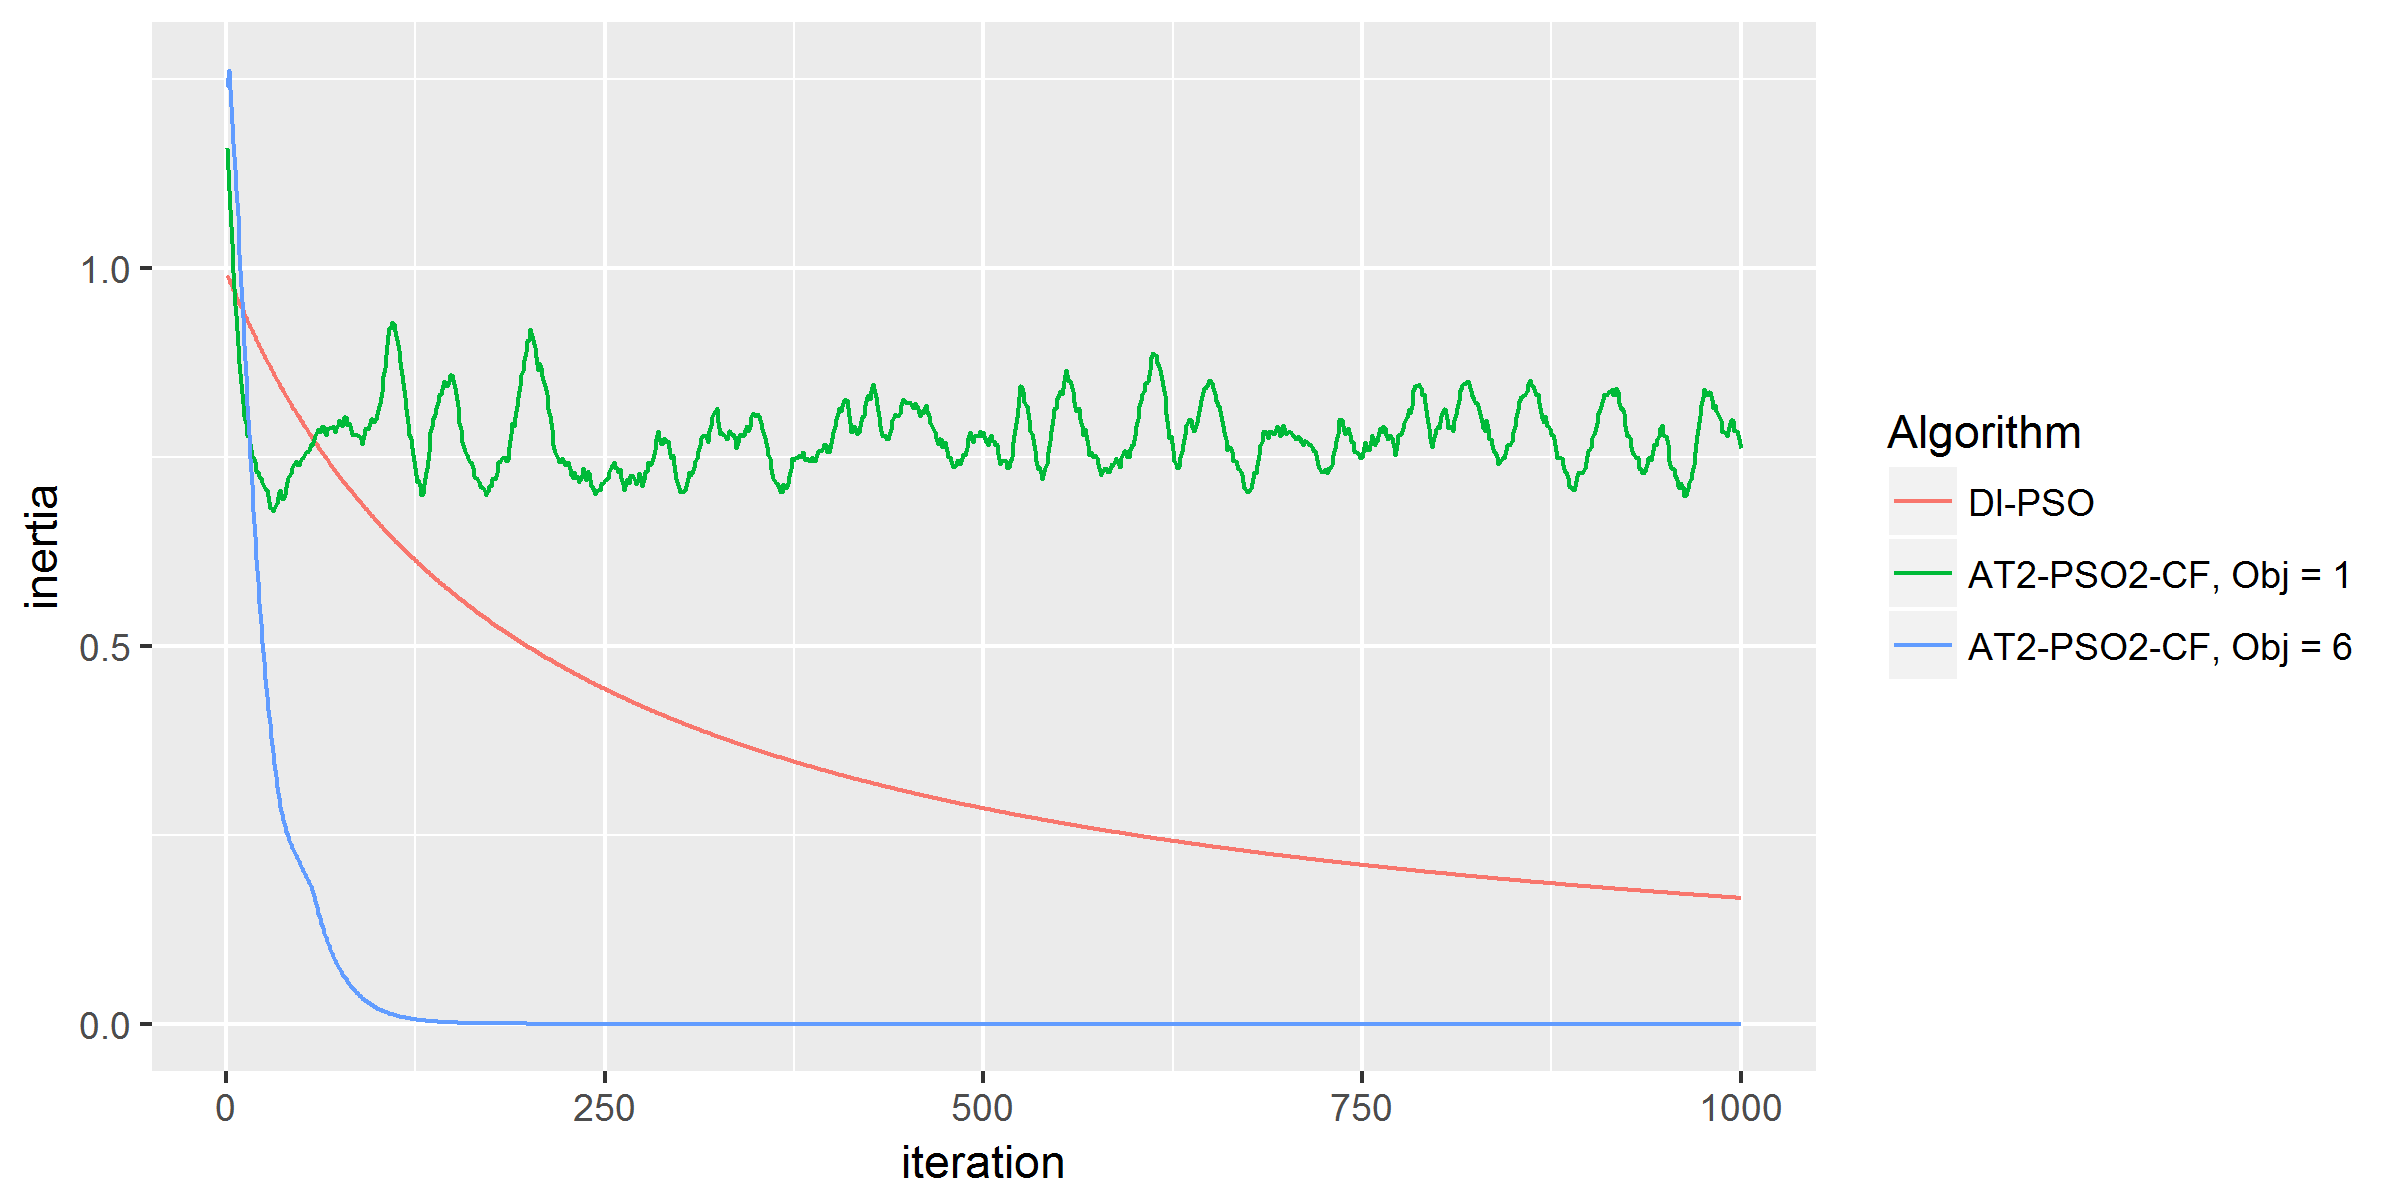
\includegraphics[width=0.95\textwidth]{../code/psosims/inertiaplot.png}
\caption{Inertia over time for the DI-PSO algorithm with $\alpha=200$ and $\beta=1$, and for one replication of the AT2-PSO-CF algorithm with the SS3 neighborhood for each of OFs 1 and 6.}
\label{fig:inertia}
\end{figure}

The AT-BBPSO algorithms are fairly competitive for most of the objective functions we consider, but AT-BBPSO strongly outperforms the alternatives in a few cases where the objective function is particularly difficult to optimize. This is clearest in Table \ref{tab:psosim6} for OF6, but in Tables \ref{tab:psosim4} and \ref{tab:psosim5} for OF5 and OF6, respectively, the best performing AT-BBPSO variants are significantly better than the best performing PSO, AT-PSO, and DI-PSO variants. AT-BBPSO algorithms also buck a couple of trends. First, the difference between the CF and non-CF variants is much less stark and is often reversed --- the best algorithms for OF6, for example, are AT-BBPSO-CF variants. Second, the SS1 neighborhood topology often works well for AT-BBPSO variants. There does not appear to be a hard and fast rule to abide by for deciding \emph{which} AT-BBPSO variant is best, but one of AT2-BBPSO-CF or AT2-BBPSOxp-CF with either the global or SS3 neighborhood tends to be the best AT-BBPSO variant for the problems we consider in this section.

Figure \ref{fig:scale} displays the scale parameter over time for one replication of the AT2-BBPSO-CF algorithm for each of the objective functions we considered with the SS3 neighborhood. Notably, they all result in similar scale parameter dynamics. This holds up remarkably well across replications, BBPSO vs. BBPSOxp, CF vs. not, and neighborhood topologies such that it may be possible to pick a one-size-fits-all deterministic progression of the scale parameter that matches the algorithm to an AT algorithm with a specific target improvement rate, $R^*$. One key source of variation that is sometimes more pronounced than in Figure \ref{fig:scale} is that for some objective functions the AT algorithms first increase the scale parameter before exponentially decaying. This flexibility to adapt to the objective function may not be worth sacrificing for the one-size-fits all approach. Rather, we highlight this possibility as a potential avenue for further understanding the AT-BBPSO algorithms.

\begin{figure}[p]
\centering
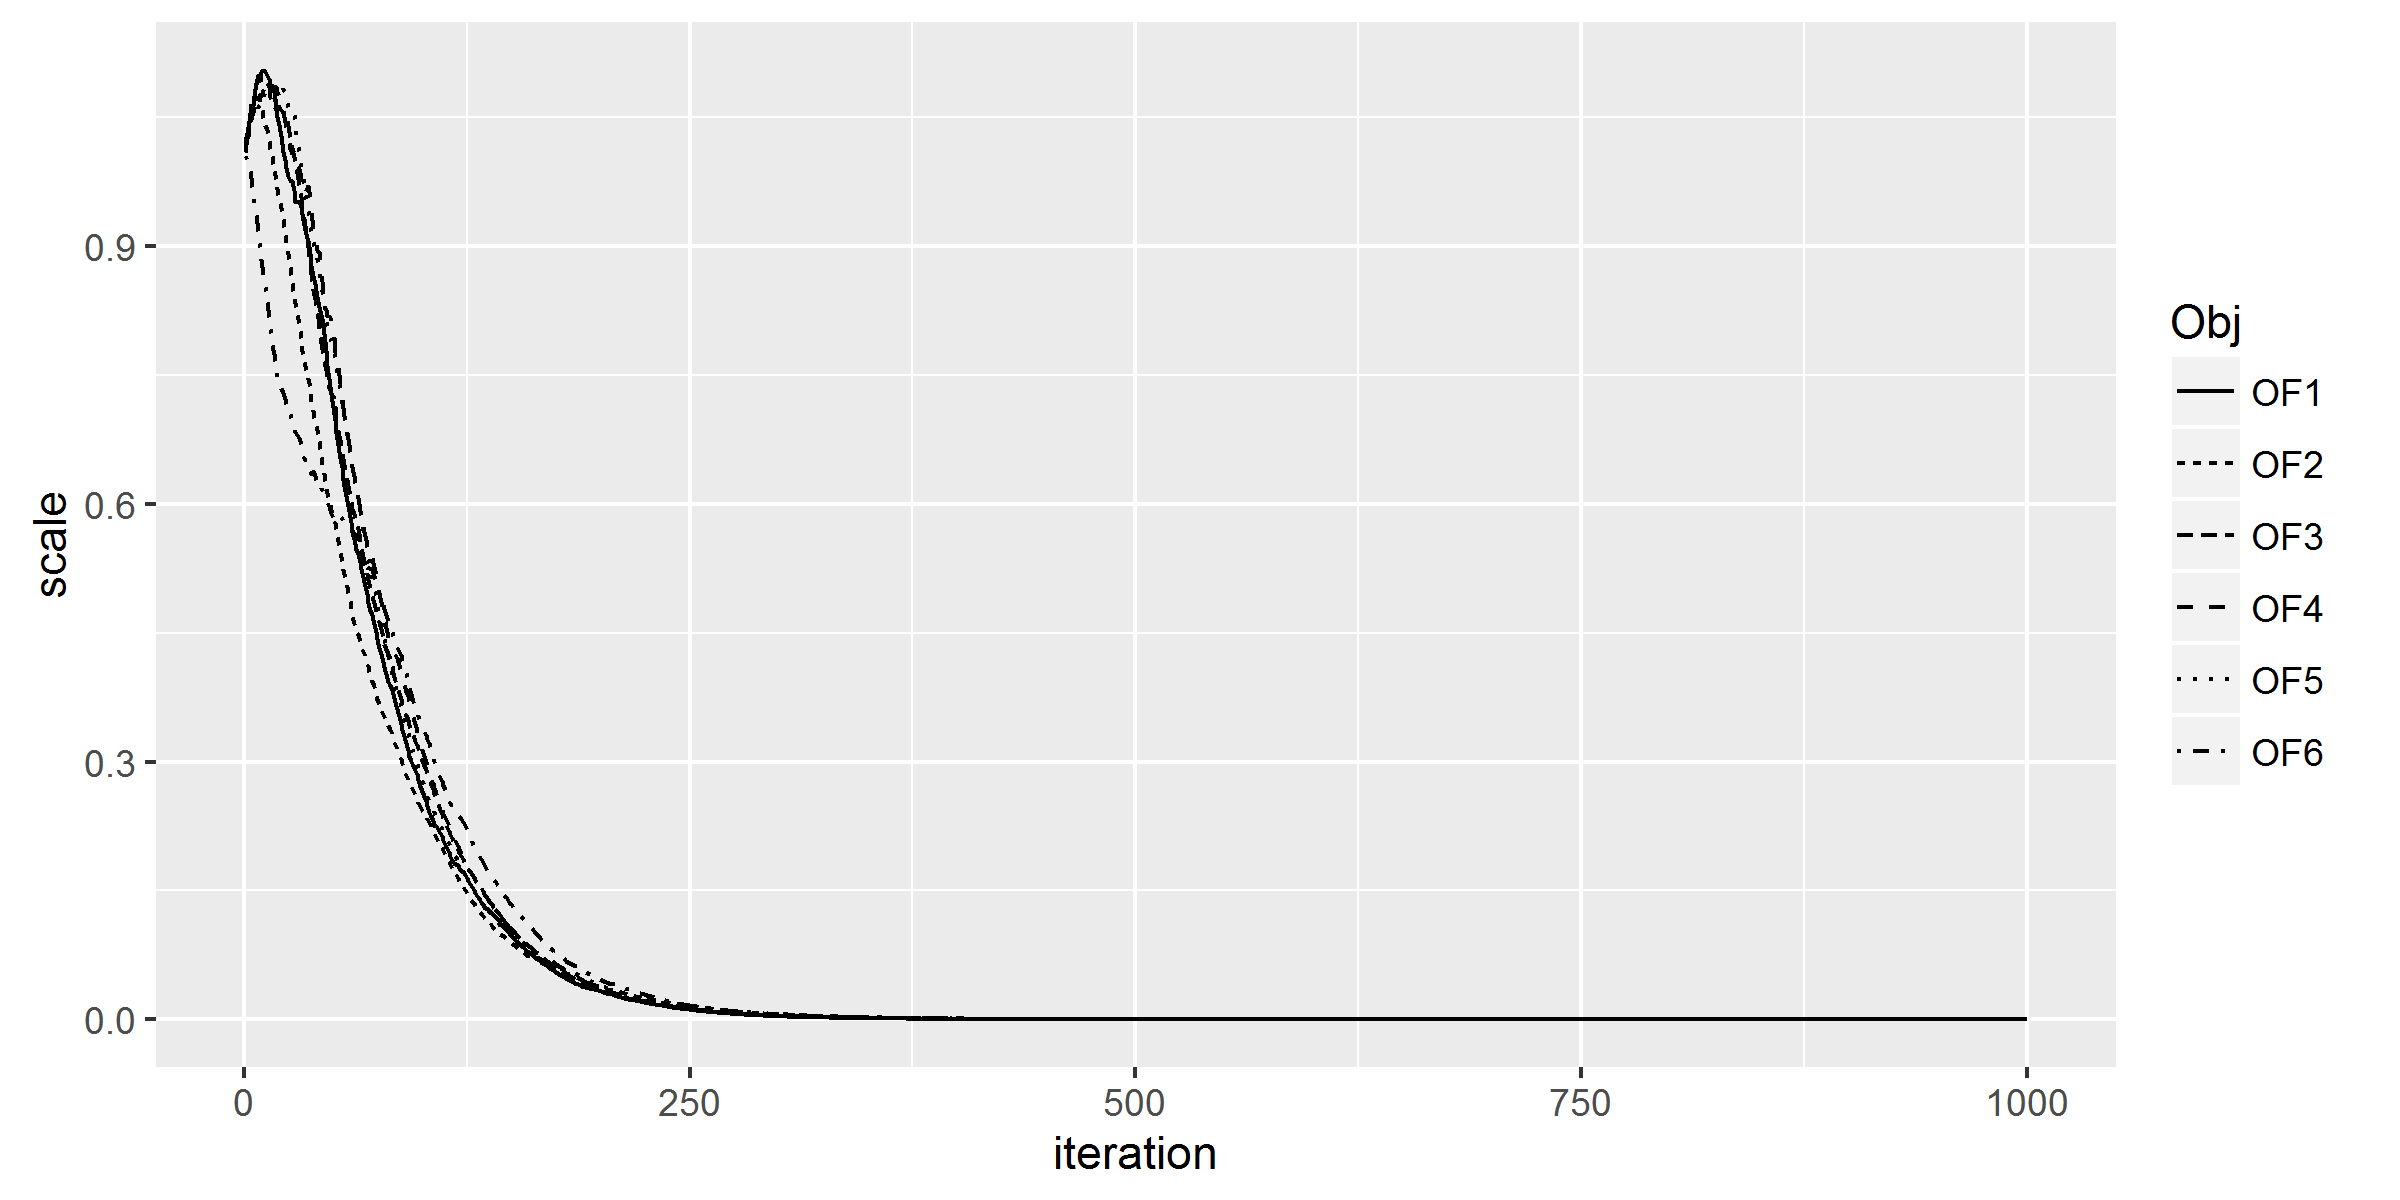
\includegraphics[width=0.95\textwidth]{../code/psosims/scaleplot.png}
\caption{Scale parameter over time for one replication of the the AT2-BBPSO-CF algorithm with the SS3 neighborhood for each of OF1--OF6.}
\label{fig:scale}
\end{figure}

AT-PSO and AT-BBPSO both improve on PSO in at least some contexts based on the results of this section. Notably for more difficult problems with, e.g., many local optima, AT-BBPSO variants are capable of vastly outperforming other PSO variants. In the next section, we turn to applying these algorithms to the practical problem of spatial network design.

\section{The Spatial Design Problem}\label{sec:spatialdesign}
Suppose we are interested in predicting a spatially indexed response variable $Y(\bm{u})$, $\bm{u}\in \mathcal{D}\subseteq \Re^2$, at a set of target locations $\bm{r}_1, \bm{r}_2, \dots, \bm{r}_{N_t}\in\mathcal{D}$ at which we seek predictions. Let $\bm{s}_1, \bm{s}_2, \dots, \bm{s}_{N_s}\in\mathcal{D}$ denote a set of $N_s$ fixed sampling locations within the spatial domain. The design problem of interest here is to add $N_d$ new sampling locations in order to optimize the amount we learn about $Y(\bm{u})$ at the target locations. See \cite{muller2007collecting}, \cite{mateu2012spatio}, and \citet[Section~11]{le2006statistical}, for general discussions of spatial design problems. Let $\bm{d}_1, \bm{d}_2, \dots, \bm{d}_{N_d}\in\mathcal{D}$ denote a set of candidate design points and suppose that $Y(\bm{u})$ is a geostatistical process with mean function $\mu(\bm{u})=\bm{x}(\bm{u})'\bm{\beta}$ for some covariate $\bm{x}(\bm{u})$ known at every point in $\mathcal{D}$ and some covariance function $C(\bm{u}, \bm{v})$ for $\bm{u},\bm{v}\in\mathcal{D}$. Typically not all covariates are known \emph{a priori} at every point in the spatial domain; however, covariates that are known functions of the location satisfy this constraint. Once the design points are selected, we observe $Z(\bm{d}_i)$ for $i=1,2,\dots,N_d$ and $Z(\bm{s}_i)$ for $i=1,2,\dots,N_s$ where $Z(\bm{u}) = Y(\bm{u}) + \varepsilon(\bm{u})$ and $\varepsilon(\bm{u})$ is mean zero white noise with variance $\tau^2$, representing measurement error and/or nugget effects. Typically $\bm{\beta}$, $\tau^2$, and $C(\cdot,\cdot)$ are unknown and must be estimated.

To completely specify the problem we need to choose an informative design criterion. Intuitively, the larger the mean square prediction error (MSPE), i.e. the kriging variance, is at each of the target locations, the less information we have about $Y(\bm{u})$ at those locations. A common design criterion is to optimize some function of these variances, e.g., to minimize the mean kriging variance or the maximum kriging variance over all target locations.

\subsection{Universal Kriging}
In classical universal kriging, $\bm{\beta}$, $\tau^2$, and the parameters of $C(\cdot,\cdot)$ are estimated, but only $\bm{\beta}$ is treated as uncertain. Let $\bm{Z}$ be the vector of $Z(\bm{s}_i)$s and $Z(\bm{d}_i)$s, $\bm{X}$ denote the corresponding stacked $\bm{x}(\bm{s}_i)'$s and $\bm{x}(\bm{d}_i)'$s, $\bm{C}_Z = \cov(\bm{Z})$ where $\cov\{Z(\bm{u}), Z(\bm{v})\} = C(\bm{u},\bm{v}) + \sigma^2_\varepsilon 1(\bm{u} = \bm{v})$, and $\bm{c}_Y(\bm{r}_i) = \cov\{Y(\bm{r}_i), \bm{Z}\}$ where $\cov\{Y(\bm{r}_i), Z(\bm{u})\} = C(\bm{r}_i, \bm{u})$. The universal kriging predictor of $Y(\bm{r}_i)$ is $\widehat{Y}_{uk}(\bm{r}_i;\bm{d}) = \bm{x}(\bm{r}_i)'\widehat{\bm{\beta}}_{gls} + \bm{c}_Y(\bm{r}_i)'\bm{C}_Z^{-1}(\bm{Z} - \bm{X}\widehat{\bm{\beta}}_{gls})$ and the MSPE of $\widehat{Y}_{uk}(\bm{r}_i)$ is
\begin{align*}
\sigma_{uk}^2(\bm{r}_i;\bm{d}) &= C(\bm{r}_i, \bm{r}_i) - \bm{c}_Y(\bm{r}_i)'\bm{C}_Z^{-1}\bm{c}_Y(\bm{r}_i)  + \{\bm{x}(\bm{r}_i)  - \bm{X}'\bm{C}_Z^{-1}\bm{c}_Y(\bm{r}_i)\}'(\bm{X}'\bm{C}_Z^{-1}\bm{X})^{-1}\{\bm{x}(\bm{r}_i)  - \bm{X}'\bm{C}_Z^{-1}\bm{c}_Y(\bm{r}_i)\}
\end{align*}
\cite[Section~4.1.2]{cressie2011statistics} where $\widehat{\bm{\beta}}_{gls} = (\bm{X}'\bm{C}_Z^{-1}\bm{X})^{-1}\bm{X}'\bm{C}_Z^{-1}\bm{Z}$ is the generalized least squares estimate of $\bm{\beta}$. For ease of notation we drop the explicit dependence on $\bm{d}$ in these equations, but $\bm{c}_Y(\bm{r}_i)$, $\bm{C}_Z$, $\bm{Z}$, $\bm{X}$, and $\widehat{\bm{\beta}}_{gls}$ all depend on $\bm{d}$. The mean universal kriging variance is given by $\overline{Q}_{uk}(\bm{d}) = \frac{1}{N_t}\sum_{i}^{N_t}\sigma^2_{uk}(\bm{r}_i;\bm{d})$ while the maximum universal kriging variance is given by $Q_{uk}^*(\bm{d}) = \max_{i=1,2\dots,N_t}\sigma^2_{uk}(\bm{r}_i;\bm{d})$. \cite{zimmerman2006optimal} finds that the optimal design under both criteria is highly dependent on the mean function of the geostatistical process. In practice we are often interested in predicting at the entire spatial domain rather than a finite set of target locations. This changes the mean and maximum kriging variances to $\overline{Q}_{uk}(\bm{d}) = \frac{1}{|\mathcal{D}|}\int_{\mathcal{D}}\sigma^2_{uk}(\bm{u};\bm{d})d\bm{u}$ and $Q_{uk}^*(\bm{d}) = \max_{\bm{u}\in\mathcal{D}}\sigma^2_{uk}(\bm{u};\bm{d})$ respectively. We can approximate both of these with a large but finite sample of target locations from $\mathcal{D}$ or a large fixed grid in $\mathcal{D}$.

\subsection{Parameter Uncertainty Kriging}
Assuming that all covariance function parameters are known, the MSPE from kriging at an arbitrary location $\bm{u}$ is $\sigma_{uk}^2(\bm{u})$. This underestimates the MSPE when those parameters must be estimated. An approximation of the correct MSPE, which we call the parameter uncertainty kriging variance (PUK variance), is given by
\begin{align*}
\E\{Y(\bm{u}) - \widehat{Y}_{uk}(\bm{u})\}^2 \approx \sigma^2_{puk}(\bm{u};\bm{d},\widehat{\bm{\theta}}) = \sigma^2_{uk}(\bm{u};\bm{d},\widehat{\bm{\theta}}) + \tr\{\bm{A}(\bm{u};\bm{d},\widehat{\bm{\theta}})\bm{I}^{-1}(\bm{d},\widehat{\bm{\theta}})\},
\end{align*}
where $\widehat{\bm{\theta}}$ is the maximum likelihood estimate of $\bm{\theta}$ from previously observed data, $\bm{I}^{-1}$ is the inverse Fisher information (FI) matrix, and $\bm{A} = \var[\partial \widehat{Y}_{uk} /\partial \bm{\theta}]$; \cite{zimmerman1992mean,abt1999estimating}. The $ij$th element of the FI matrix can be derived as $\tr\left(\bm{C}_Z^{-1}\frac{\partial\bm{C}_Z}{\partial\theta_i}\bm{C}_Z^{-1}\frac{\partial\bm{C}_Z}{\partial\theta_j}\right)$ while $\bm{A}$ can be derived using elementary matrix calculus. From these we define the mean and maximum  PUK variances as $\overline{Q}_{puk}(\bm{d}) = \frac{1}{N_t}\sum_{i}^{N_t}\sigma^2_{puk}(\bm{r}_i;\bm{d})$ and $Q_{puk}^*(\bm{d}) = \max_{i=1,2\dots,N_t}\sigma^2_{puk}(\bm{r}_i;\bm{d})$, respectively.

\subsection{Houston Ozone Monitoring}\label{sec:houston}
A 20 parts per billion (ppb) increase in daily maximum eight-hour ozone concentration (DM8) has been associated with an increased risk of out-of-hospital cardiac arrest, with a relative risk estimate of 1.039; \cite[95\% CI {[}1.005, 1.073{]},][]{ensor2013case}. The Texas Commission on Environmental Quality (TCEQ) has monitoring stations throughout Texas recording Ozone levels, along with a variety of other environmental indicators. The TCEQ measures ozone at a network of monitoring locations and publishes DM8s in ppb for each monitoring location. The DM8s are computed as follows. First, the TCEQ creates an hourly mean in ppb for each monitoring location. Then they construct an eight hour mean at that location for each contiguous eight-hour period where all eight measurements were present for a given day. The maximum of these eight-hour means for a given day is the published DM8. Days with less than 18 valid eight-hour means have no published DM8.

In August 2016 there were 44 active monitoring locations in the Houston-Galveston-Brazoria area, which we focus on. For each location $\bm{u}$ we compute the monthly mean DM8, which we denote by $Z(\bm{u})$. At one location, MRM-3 Haden Road, there are two DM8 observations of zero ppb in the month of August. We assume that these were data errors and omit them for the purposes of computing $Z(\bm{u})$ at that location. Of the 44 locations, one has 15 valid DM8 measurements of 31 possible valid measurements, another has 24 valid measurements, and the rest of the locations have at least 27 valid measurements.

The hypothetical design problem we consider is the addition of 100 new ozone monitoring locations to the Houston-Galveston-Brazoria monitoring network in Harris County, where Houston is located, with the goal of predicting ozone concentrations within the county. Harris County contains 33 of the 44 existing locations, though the locations outside of the county are still useful for spatial prediction within the county.

Let $Z(\bm{u})$ denote the measured mean DM8 at location $\bm{u}$ and let $Y(\bm{u})$ denote the true DM8. We assume that $Z(\bm{u})$ is a noisy measurement of $Y(\bm{u})$ with the data model $Z(\bm{u}) \sim N[Y(\bm{u}), \tau^2]$. The parameter $\tau^2$ represents variability added due to measurement error from the instruments, small-scale effects, and potentially sampling error from measuring DM8 on less than the full 31 days in August. At the process level, we assume that $Y(\bm{u})$ is a Gaussian process with mean function $\mu(\bm{u}) = \bm{x}(\bm{u})'\bm{\beta}$ and exponential covariance function $C(\bm{u},\bm{v}) = \sigma^2\exp(-||\bm{u} - \bm{v}||/\psi)$. We considered several possible mean functions: constant in $\bm{u}$, linear in $\bm{u}$, and quadratic in $\bm{u}$. We fit each model using maximum likelihood and found that quadratic terms were unnecessary, but linear terms did significantly help explain variation in $Y(\bm{u})$.

We use both PUK design criteria defined in Section \ref{sec:spatialdesign} in order to choose the 100 new monitoring locations in Harris County, namely $\overline{Q}_{puk}(\bm{d})$ and $Q^*_{puk}(\bm{d})$. We assume that the goal is to predict mean DM8 in all of Harris County, so we approximate the continuous versions of $\overline{Q}_{puk}(\bm{d})$ and $Q^*_{puk}(\bm{d})$ with the finite sample versions using a grid of 1229 points, obtained by gridding up the smallest rectangle containing Harris County and throwing away all points outside of the county. We try a variety of PSO algorithms in order to select the new locations. Since the design space only allows new monitoring locations within Harris County, we modify each of the PSO algorithms we use so that any particle outside of the design space is forced to moved to the nearest point on the edge of the design space using the \verb0gNearestPoint0 function from the \verb0rgeos0 \verb0R0 package \citep{rgeos2016, R2016}. Existing sampling locations outside of Harris County are still used in the estimation of the model and in the construction of the PUK variances.

Table \ref{tab:psokriging} contains the results of applying each optimization algorithm to choosing the 100 new monitoring locations once with each algorithm. In the table, PSO refers to the standard PSO algorithm with the usual velocity update and all of the other modifications listed in Section \ref{subapp:pso} of the supporting materials. The CF modifier indicates that the velocity update is coordinate-free -- see Section \ref{subapp:pso} for details. The AT modifier indicates that $\omega(k)$ is adaptively tuned as described in Section \ref{sec:AT-PSO}. AT1 uses $R^*=0.3$ and AT2 uses $R^*=0.5$, while both use $c=0.1$ and $\omega(0) = 1.2$. We use two sets of parameter values for all of the PSO algorithms: $\phi_1^{(1)}=\phi_2^{(1)}=1.496$ (PSO1) and $\phi_1^{(2)}=\phi_2^{(2)}=\ln(2) + 1/2$ (PSO2), and when applicable the corresponding inertias are $\omega^{(1)}=0.7298$ and $\omega^{(2)}=1/(2\ln 2)$. We do not list any DI algorithms since they performed extremely poorly on this problem. All of the BBPSO algorithms we consider are AT, with AT1-BBPSO and AT2-BBPSO using the same parameter values of $R^*$, and $c$ as AT1-PSO and AT2-PSO respectively. All BBPSO algorithms also use $df=1$, and each of the modifications detailed in Section \ref{subapp:bbpso} of the supporting materials. Further, the CF modifier indicates that the BBPSO algorithm uses the coordinate-free variance update and the xp modifier indicates it has a 0.5 probability of moving any given coordinate of a particle to its personal best location on that coordinate, both described in Section \ref{subapp:bbpso}. All of the PSO and BBPSO algorithms use the global neighborhood topology. In simulations not reported here, we found that the stochastic star topology resulted in worse PSO algorithms for the spatial design problem, so we limit our attention to the global topology. Further, each PSO algorithm has a swarm size of 40, which is the standard value proposed by \cite{clerc2011spso}. We run each PSO algorithm for $K=2000$ iterations, which is roughly when most of them seemed to settle down and stop improving.

Additionally, we employ a class of genetic algorithms (GAs) described in \cite{hamada2001finding} to compare to PSO, with one batch, and with two possible mutation rates ($\lambda_1 = 0.01$ or $\lambda_2 = 0.1$) and two possible mutation variances ($\mu_1 = 1$ or $\mu_2 = 2$). The GAs also use a population of 40, though they are only allowed to run for 1000 iterations so that after the initialization, the GAs use the same number of objective function evaluations as each of the PSO algorithms. In order to handle the bounded search space, we use the same method for the GAs as for the PSO algorithms described in Section \ref{app:psodetail} of the supporting materials: any point the GA suggests that is outside of Harris County is moved to the nearest point on the border of the county. Each algorithm was implemented in the \verb0R0 programming language \citep{R2016}. In Table \ref{tab:psokriging}, GAs are referred to by ``GA-$ab$'' where $a$ denotes which value of $\lambda$ is used and $b$ denotes which value of $\mu$ is used. As a point of comparison for both classes of algorithms, we randomly selected the 100 new monitoring locations uniformly from Harris county 10,000 times independently and computed the values of $\overline{Q}_{puk}$ and $Q^*_{puk}$. The means of these values are labeled as ``Uniform'' in Table \ref{tab:psokriging}.

% latex table generated in R 3.3.2 by xtable 1.8-2 package
% Tue Jan 03 15:55:01 2017
\begin{table}[p]
\centering
\begingroup\scriptsize
\begin{tabular}{lrr}
Algorithm & $\overline{Q}_{puk}$ & $Q^*_{puk}$ \\\hline
Uniform & 16.40 & 26.80 \\\hline
PSO1 & \bf{14.40} & \bf{20.63} \\
  PSO2 & 14.45 & \bf{21.03}\\
  PSO1-CF & 15.53 & 23.54 \\
  PSO2-CF & 15.77 & 23.16 \\
   \hline
AT1-PSO1 & \bf{14.38} & \bf{20.57} \\
  AT1-PSO2 & 14.56 & 23.18 \\
  AT1-PSO1-CF & 15.96 & 23.33 \\
  AT1-PSO2-CF & 15.60 & 24.02 \\
   \hline
AT2-PSO1 & \bf{14.42} & \bf{21.13} \\
  AT2-PSO2 & \bf{14.32} & 22.11 \\
  AT2-PSO1-CF & 15.85 & 24.00 \\
  AT2-PSO2-CF & 15.95 & 23.63 \\
   \hline
AT1-BBPSO & 14.53 & 22.28 \\
  AT1-BBPSOxp & 15.87 & 22.19 \\
  AT1-BBPSO-CF & 14.65 & 21.33 \\
  AT1-BBPSOxp-CF & 14.84 & 22.34 \\
   \hline
AT2-BBPSO & 14.65 & 23.49 \\
  AT2-BBPSOxp & 15.21 & 23.25 \\
  AT2-BBPSO-CF & 14.63 & 21.92\\
  AT2-BBPSOxp-CF & 14.52 & 22.76 \\
   \hline
GA-11 & \bf{14.40} & 21.19 \\
  GA-21 & 15.20 & 23.21 \\
  GA-12 & 14.45 & \bf{20.84} \\
  GA-22 & 15.26 & 22.61 \\
\hline
\end{tabular}
\endgroup
\caption{ Simulation results for each objective function, $\overline{Q}_{puk}$ and $Q^*_{puk}$. Bolded values in a given column are the five best (lowest)  values for the corresponding objective function. AT-PSO and AT-BBPSO variants are adaptively-tuned, with AT1 and AT2 corresponding to two different parameter settings for the tuned portion of the algorithm. CF indicates that the velocity or scale parameter update is coordinate free. PSO1 and PSO2 use two different parameter settings for any non-adaptive parameters, and similarly for BBPSO and BBPSOxp. GAs have two possible values for a rate parameter and also for a variance parameter, indicated by the appended numbers. See text for further description of all of these parameter settings.}
\label{tab:psokriging}
\end{table}

From Table \ref{tab:psokriging} we immediately see that the first set of parameter values tends to work the best in the PSO algorithms, while in the AT-BBPSO algorithms the non-xp variants tend to outperform the xp variants, though neither of these is universally true. For both objective functions the PSO1 algorithm with the global neighborhood topology performs the best of the standard PSO variants and is outperformed by several of the AT variants. The best GAs are competitive with the best PSO algorithms, though they appear to be slightly worse. The five best performing algorithms for $\overline{Q}_{puk}$ are, in order, AT2-PSO2, AT1-PSO1, GA-11, PSO1-Global, and AT2-PSO1 (bold in Table \ref{tab:psokriging}). Similarly, the five best performing algorithms for $Q^*_{puk}$ are, in order, AT1-PSO1, PSO1, GA-12, PSO2, and AT2-PSO1 (bold in Table \ref{tab:psokriging}). In Section \ref{sec:psocompare} we found that the AT-BBPSO and AT-BBPSO-CF variants were competitive with the other PSO algorithms and in the case of the hardest problems seemed to be the best. The key seems to be that the AT-BBPSO variants are more robust to complicated objective surfaces with many local minima. When the objective surface is simpler, PSO and AT-PSO variants are more attractive and appear to converge faster. Similarly, for problems that are simple enough PSO outperforms AT-PSO, but for hard enough problems AT-PSO becomes advantageous. For example, in simulations not reported here, PSO1 outperforms all other algorithms when adding significantly less monitoring locations to the network, e.g., 20. But in this case, with 100 new locations, AT1-PSO1 appears to be superior for both objective functions, though the difference is small.

\begin{figure}[p]
\centering
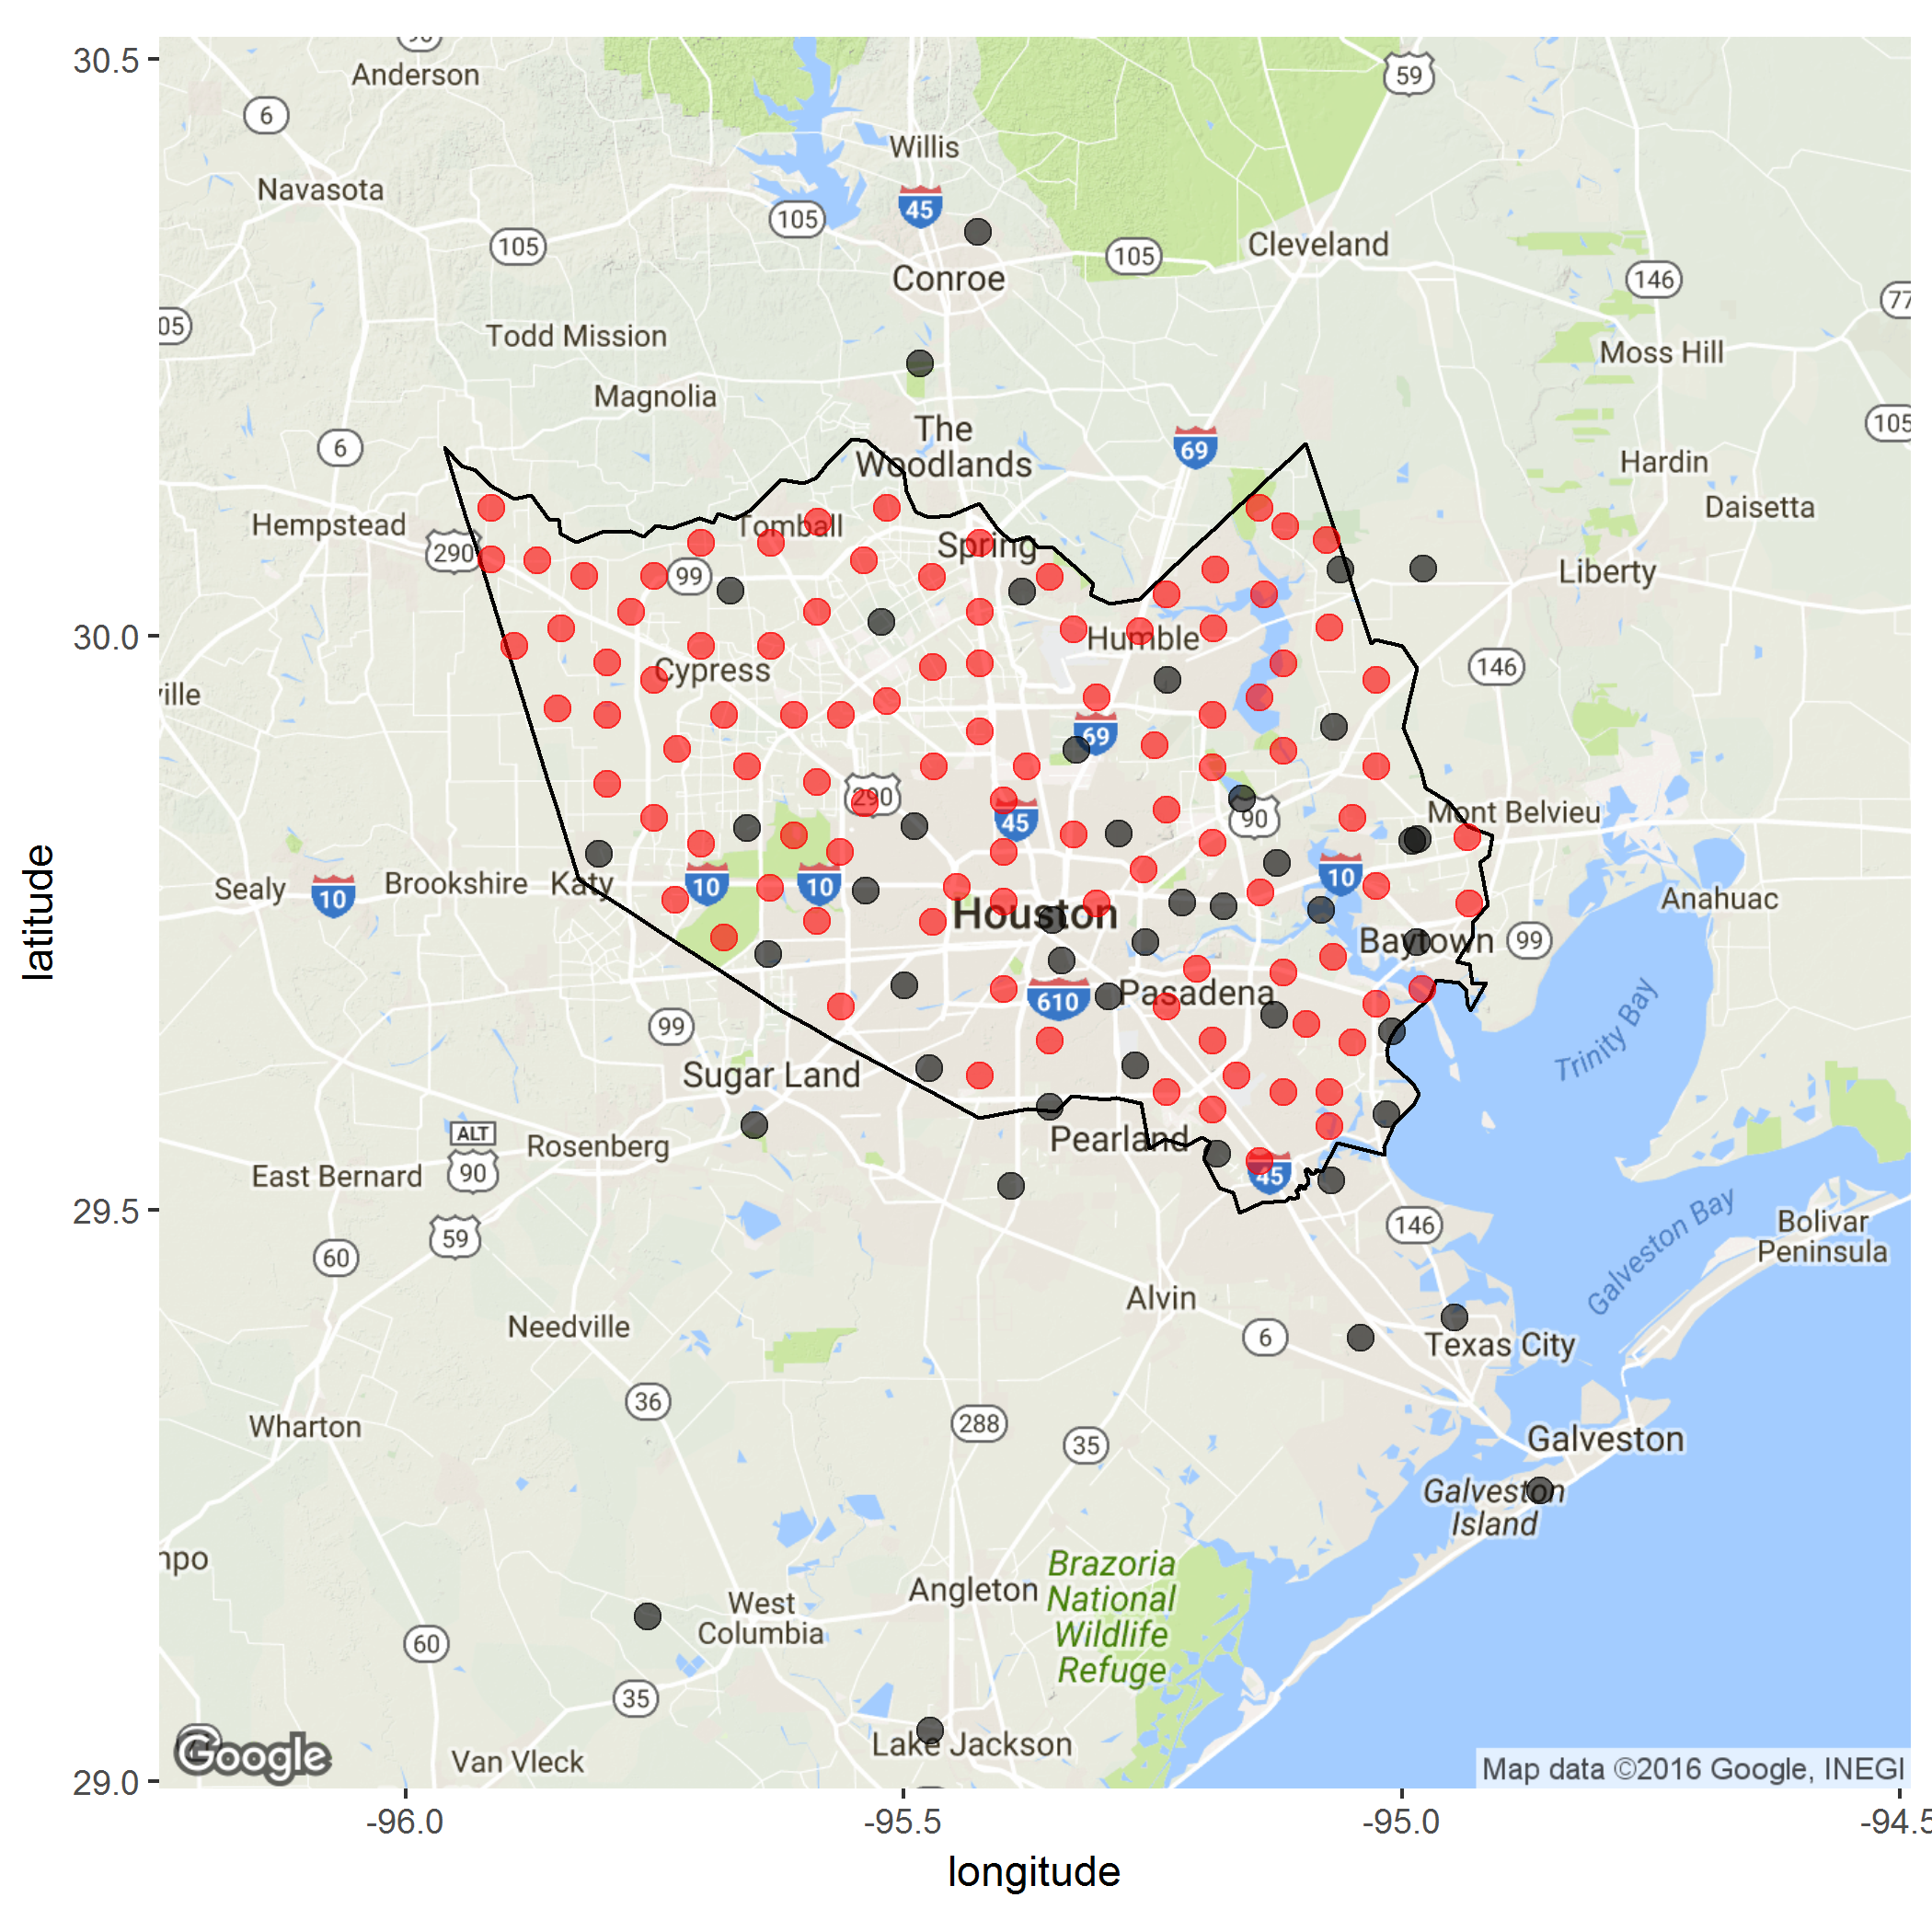
\includegraphics[scale=.8]{../code/kriging/sig2pukmean.png}
\cprotect\caption{Best designs found according to $\overline{Q}_{puk}$. Original network points are gray, new points are red. Harris County is outlined in black. The background map is from Google Maps via \verb0ggmap0; \cite{ggmap2013}.}
\label{fig:designoutmean}
\end{figure}

\begin{figure}[p]
\centering
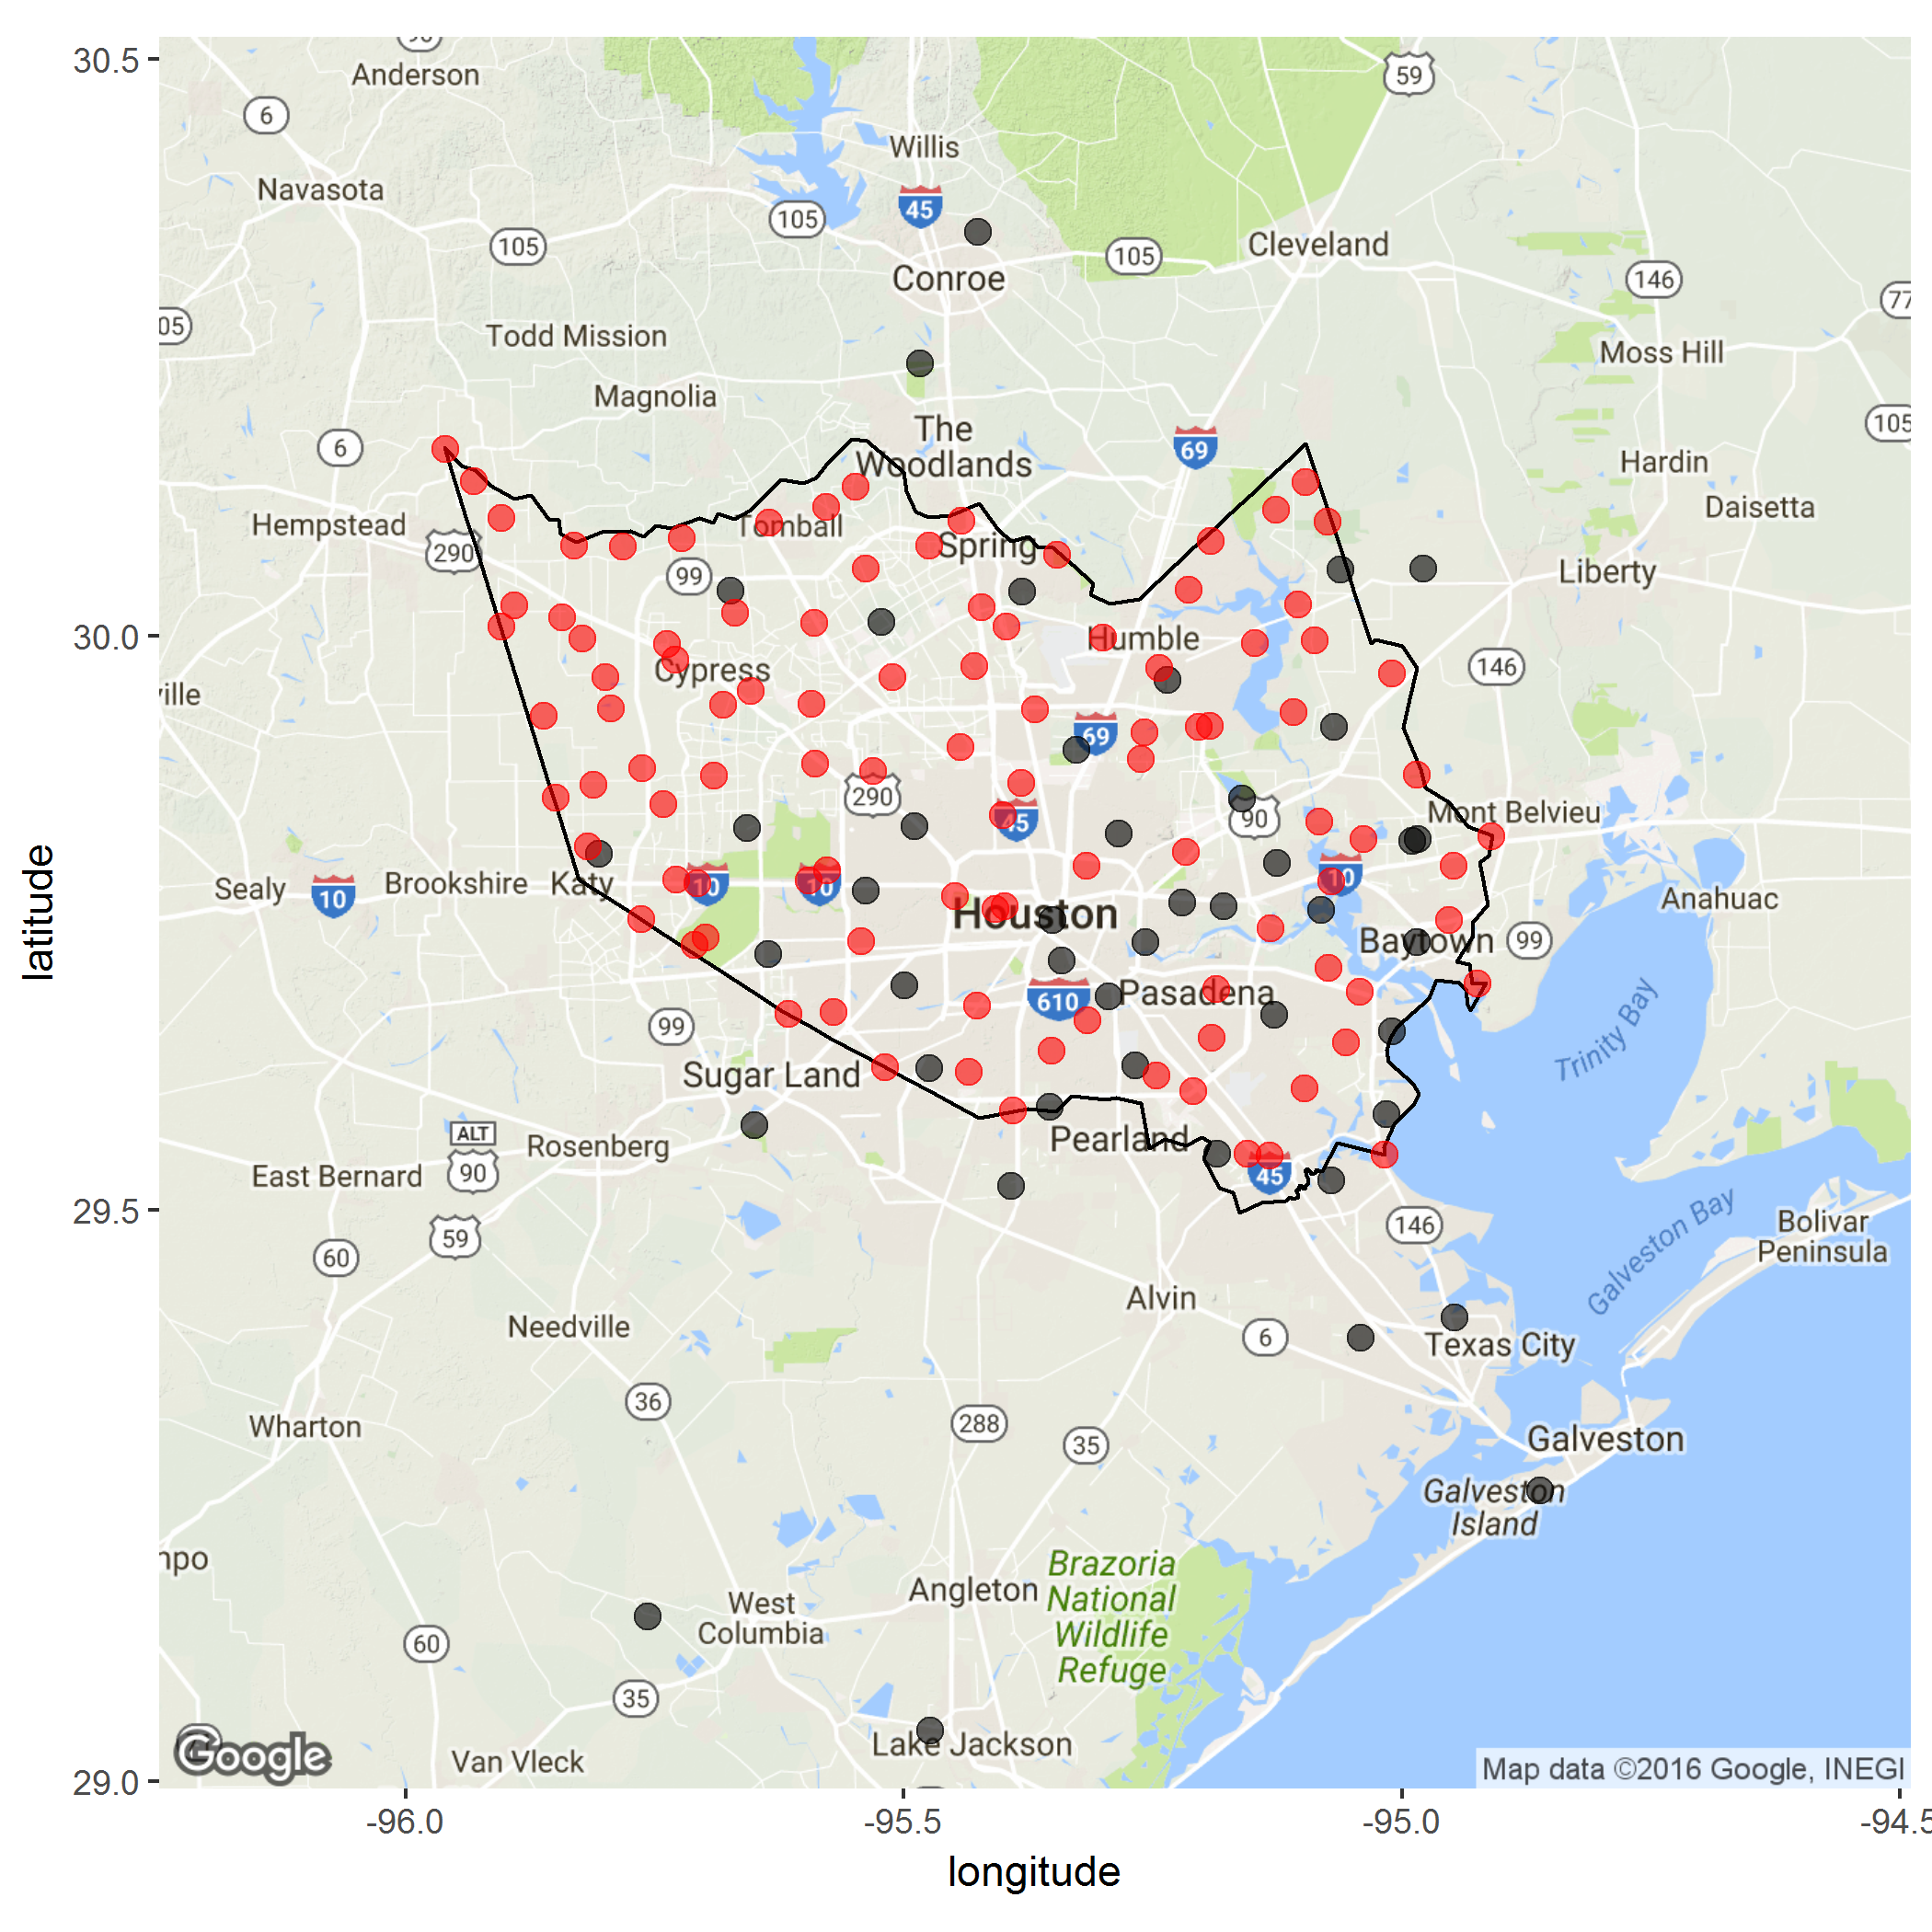
\includegraphics[scale=.8]{../code/kriging/sig2pukmax.png}
\cprotect\caption{Best designs found according to $Q^*_{puk}$. Original network points are Gray, new points are red. Harris County is outlined in black. The background map is from Google Maps via \verb0ggmap0; \cite{ggmap2013}.}
\label{fig:designoutmax}
\end{figure}

Figures \ref{fig:designoutmean} and \ref{fig:designoutmax} contain the best designs found using $\overline{Q}_{puk}$ and $Q^*_{puk}$, respectively. When using the mean kriging variance ($\overline{Q}_{puk}$), the best design spreads nodes of the network fairly evenly throughout the spatial domain. With the maximum kriging variance ($Q^*_{puk}$), the best design is more erratic. Notably, there are many more nodes directly on or very close to the border of the spatial domain while interior areas have a tendency to be more sparsely populated with nodes. This is unsurprising since $Q^*_{puk}$ is worst case kriging variance over the entire county, which incentivizes obtaining a better estimate of $\bm{\beta}$. The further away a point is from other monitoring locations, the more the prediction depends on the model's estimate of $\bm{\beta}$ and the less it depends on the values of nearby observations, and putting more monitoring locations near the edges of the county results in smaller variances for the elements of $\widehat{\bm{\beta}}_{gls}$.

\section{Discussion}\label{sec:discuss}

In this paper we reviewed PSO algorithms, introduced AT-PSO and AT-BBPSO algorithms, and demonstrated that PSO, AT-PSO, and AT-BBPSO algorithms are useful for spatial design problems. In the simulation study in Section \ref{sec:psocompare} we found that AT-BBPSO variants were especially attractive for optimization problems with complicated objective surfaces, potentially with many local optima. However, in Section \ref{sec:houston} we found little difference between the standard PSO algorithm and the best AT algorithms. The upshot is that at least for spatial design problems similar to or easier than the one we considered here, using a standard PSO algorithm with standard parameter settings and the typical modifications we list in Section \ref{subapp:pso} is a good default, especially since this algorithm is already implemented in several widely available packages such as the \verb0pso0 package in \verb0R0 \citep{bendtsen2012pso}. Furthermore, in similar spatial design problems which are much lower dimensional than the one discussed in this paper we have found that standard PSO algorithms are often the best.

However, our results in Section \ref{sec:psocompare} suggest that with more complex objective functions there may be significant benefits to using AT-BBPSO. In the hardest problems, AT-BBPSO variants were significantly better than the alternatives. In our spatial design problem in Section \ref{sec:houston}, the best performing algorithms were AT-PSO variants, though the difference was small. This is consistent with our results in Section \ref{sec:psocompare} where occasionally an AT-PSO variant was the best for one of the simpler objective functions, but usually not by much. Compared to the design problem we considered, additional objective function complexity may come from a more complex spatial model with a more complex mean or covariance function, or a more complex design criterion such as an entropy based criterion. As long as the user has a reasonable expectation that the objective surface is not too complex, whichever algorithm is easier for them to implement and use is likely the best, but for more complex problems there is much to be gained from trying several different algorithms and in particular from the AT-BBPSO variants we introduced.

The usefulness of PSO and AT variants for statistics is not limited to spatial design. Other design problems are amenable to PSO; for example, the problem of which blocks to select in the context of address canvassing, e.g. see \cite{young2016zero}, after determination of coverage errors. In general, any optimization problem which is difficult to solve with gradient based algorithms is a good candidate, especially when near-optimal solutions are tolerable. In the spatial design literature, exchange algorithms are commonly employed instead of PSO or GAs, though these require limiting the search space to a discrete grid; \cite{nychka1998design,wikle1999space,wikle2005dynamic}. PSO (and GA) allow the entire search space to be used without restriction and are attractive for this reason, though in cases where there is a known discrete set of possible monitoring locations the exchange algorithm is more suited to the task.

\ack{This report is released to inform interested parties of research and to encourage discussion.  The views expressed on statistical issues are those of the authors and not necessarily those of the U.S. Census Bureau.}

\bibliographystyle{wb_stat}
\bibliography{pso}
\end{document}


